%%%%%%%%%%
\section{Limitations of the standard model}
\label{sec:SMLimitations}
%%%%%%%%%%

The standard model has been remarkably confirmed by experimental data collected over the last few decades, which validated all its predictions.
The ultimate verification of the model has been provided by the latest discovery of a scalar particle at the LHC (Section~\ref{subsec:HiggsLHC}), whose properties are largely compatible with the SM predictions for the Higgs boson.
Nevertheless, there are fundamental physical phenomena in nature that cannot be adequately explained by the SM. %as well as theoretical deficiencies that make the model unsatisfactory.
Furthermore, some features of the model represent \textit{ad hoc} additions to the theory and, although providing predictions that have been confirmed, imply a lack of understanding, making the framework theoretically unsatisfactory.
Some of the main unresolved issues of the SM are briefly described in the following.

\subsection*{The hierarchy problem}

This issue arises from the observation of a large discrepancy between the electroweak and gravity scales. This is reflected in the mass difference between the masses of the \PW and \PZ bosons that define the scale of electroweak interactions ($\mathcal{O}(10^2\GeV)$), and the Planck mass ($\MPl = \sqrt{\hbar c/G_\mathrm{Newton}} = \mathcal{O}(10^{19})$), that defines the scale beyond which gravity must be described by quantum mechanics. This feature is commonly known as \textit{hierarchy problem} or as well ``problem of \textit{naturalness}'', meaning an ``unnatural'' or equivalently ``unexpected'' behaviour.
More technically, the question is why the Higgs boson of mass $m_\PH$ (Eq.~\ref{eqn:SM_e38}) is so much lighter than the Planck mass.
%\begin{wrapfigure}{R}{0.4\textwidth}
 %\centering
 %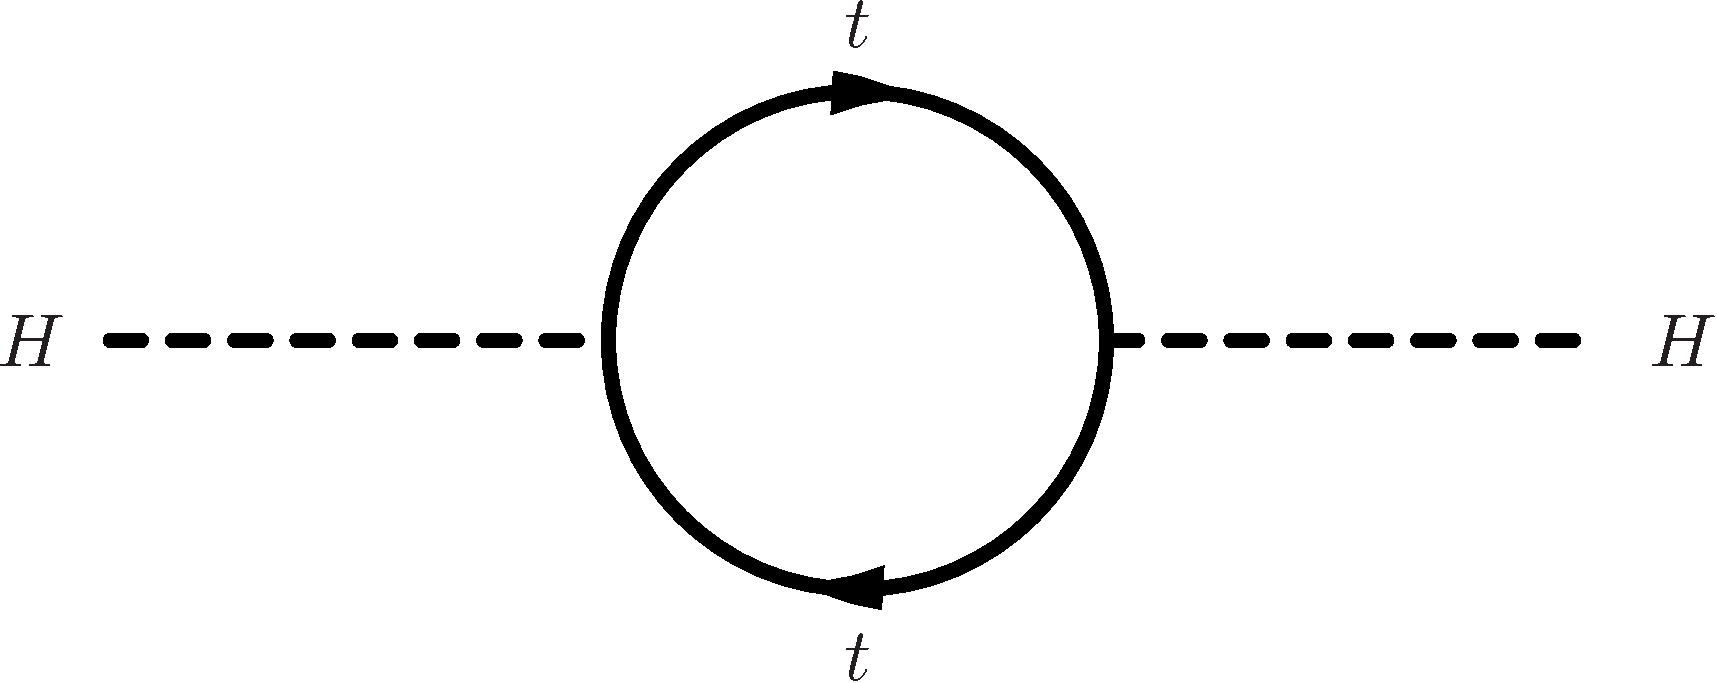
\includegraphics[width=0.35\textwidth]{\chtwo/HiggsLoop.pdf}
 %\caption{One-loop quantum corrections to the Higgs squared mass parameter $m^2_\PH$ due to a fermion $f$.}
 %\label{fig:HiggsLoop}
%\end{wrapfigure}
The problem is that $m^2_\PH$ receives enormous quantum corrections from the virtual effects of every particle that couples, directly or indirectly, to the Higgs field.
%For example, the Feynman diagram in Fig.~\ref{fig:HiggsLoop} brings a correction to $m^2_\PH$ from a loop containing a fermion $f$ with mass $m_f$.
%If the Higgs field $H$ couples to $f$ with a term in the Lagrangian $-\lambda_fH\bar{f}f$, where $\lambda_f$ is the Yukawa coupling, then this loop yields a correction
%\begin{equation}\label{eqn:HiggsCorr}
%\delta m^2_\PH = - \frac{|\lambda_f|^2}{8\pi^2}\Lambda^2 + \dotsc,
%\end{equation}
%\noindent where $\Lambda$ is a momentum cut-off representing the scale up to which the SM remains valid, and beyond which new physics enters to alter the high-energy behavior of the theory.
There are three types of radiative corrections to the Higgs mass that arise from the diagrams in Fig.~\ref{fig:HiggsLoop}.
Each of them gives a correction to the Higgs mass:

\begin{equation}\label{eqn:HiggsCorr}
\begin{aligned}
\mbox{top loop} & \qquad\qquad\qquad\qquad -\frac{3}{8\pi^2}\lambda_t\Lambda^2\\
\mbox{gauge loop} & \qquad\qquad\qquad\qquad + \frac{1}{16\pi^2}g^2\Lambda^2\\
\mbox{Higgs loop} & \qquad\qquad\qquad\qquad + \frac{1}{16\pi^2}\lambda^2\Lambda^2\\
\end{aligned}
\end{equation}

\noindent where $\Lambda$ is a momentum cut-off representing the scale up to which the SM remains valid, and beyond which new physics enters to alter the high-energy behavior of the theory.
Each of the leptons and quarks of the SM also contribute, however the largest correction arises from the top quark.
%Each of the leptons and quarks of the SM can play the role of $f$ and the largest correction arises when $f$ is the top quark.
If $\Lambda$ is of the order of \MPl, then this quantum correction to $m^2_\PH$ is about 30 orders of magnitude larger than the measured value of $m_\PH$ of 125\GeV.
Thus, in order to obtain such a small value for the Higgs boson mass an incredible fine-tuning cancellation must occur between the quadratic radiative corrections and the physical mass.
Avoiding such a miraculous cancellation can only happen if the cut-off scale $\Lambda \simeq \mathcal{O}(1 - 10\TeV)$ rather than the Planck scale, that is, if new physics shows up at that energy.
This is only directly a problem for corrections to the Higgs scalar boson squared mass, because quantum corrections to fermion and gauge boson masses do not have the direct
quadratic sensitivity to $\Lambda$ found in Eq.~\ref{eqn:HiggsCorr}. However, the quarks and leptons and the electroweak gauge bosons of the SM all obtain masses from the Higgs boson,
so that the entire mass spectrum of the theory is directly or indirectly sensitive to the cut-off $\Lambda$.

\begin{figure}[!htb]
 \centering
 \subfigure[]{\label{fig:HiggsLoop_a}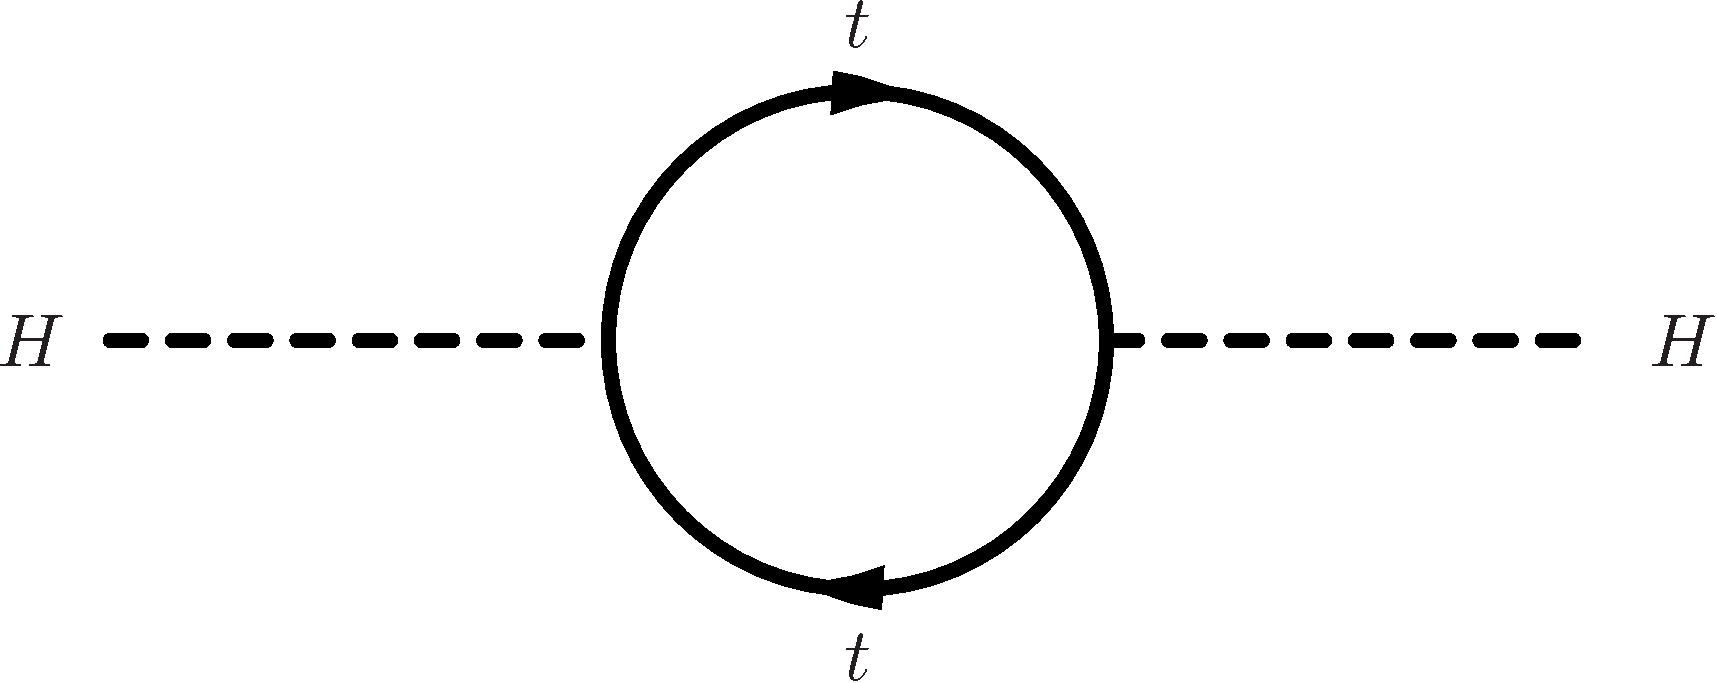
\includegraphics[width=0.3\textwidth]{\chtwo/HiggsLoop.pdf}}
 \subfigure[]{\label{fig:HiggsLoop_b}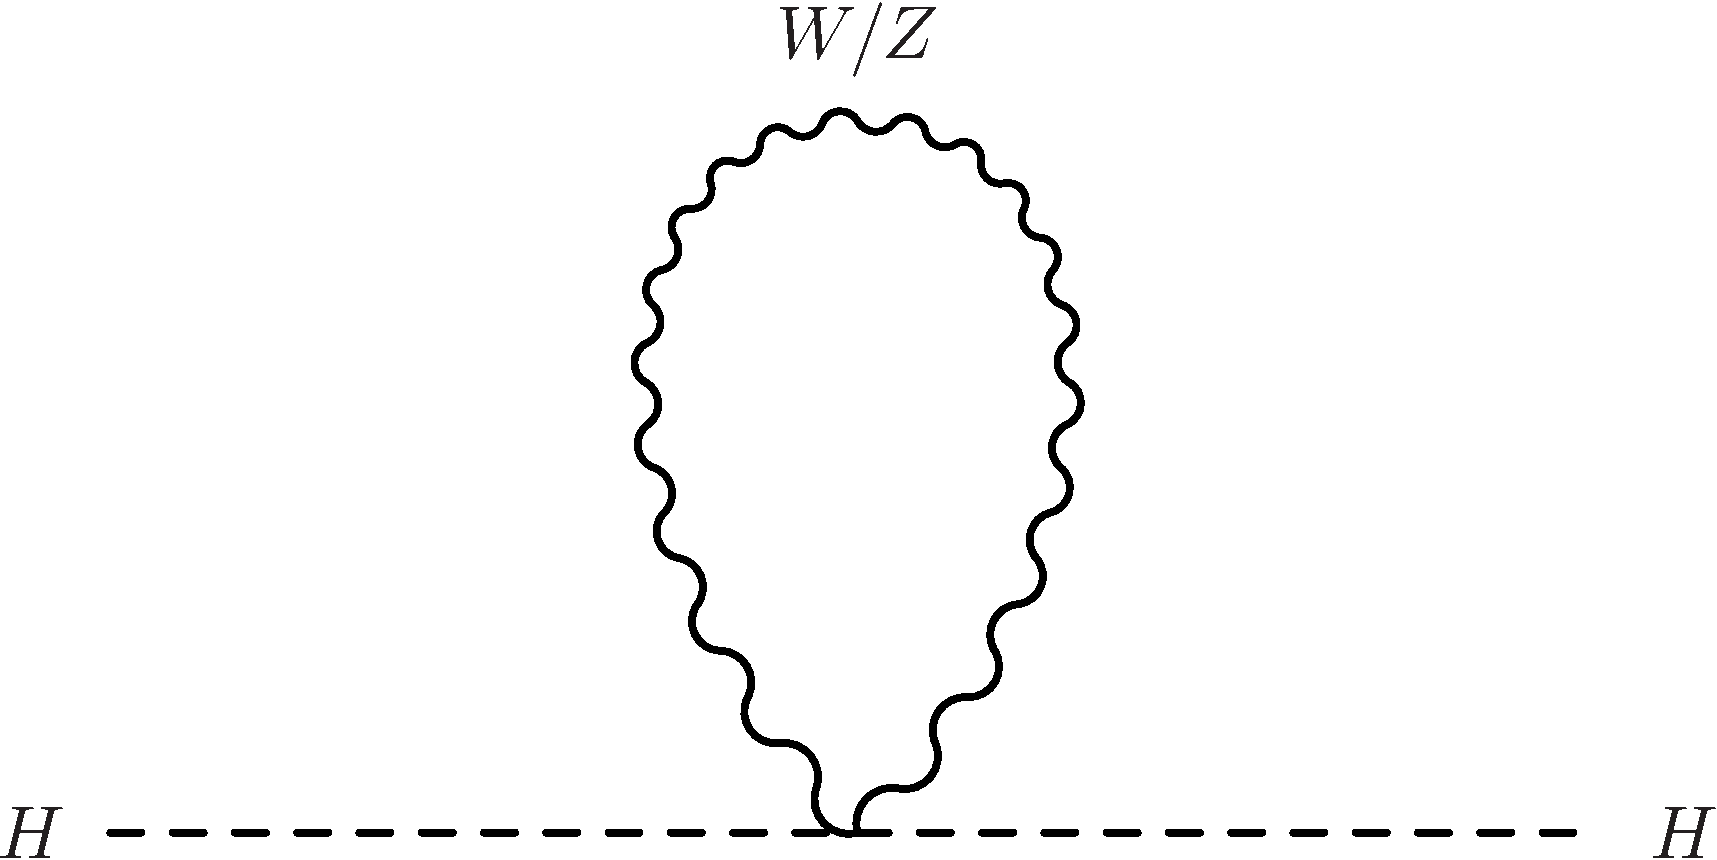
\includegraphics[width=0.3\textwidth]{\chtwo/HiggsLoop1.pdf}}
 \subfigure[]{\label{fig:HiggsLoop_c}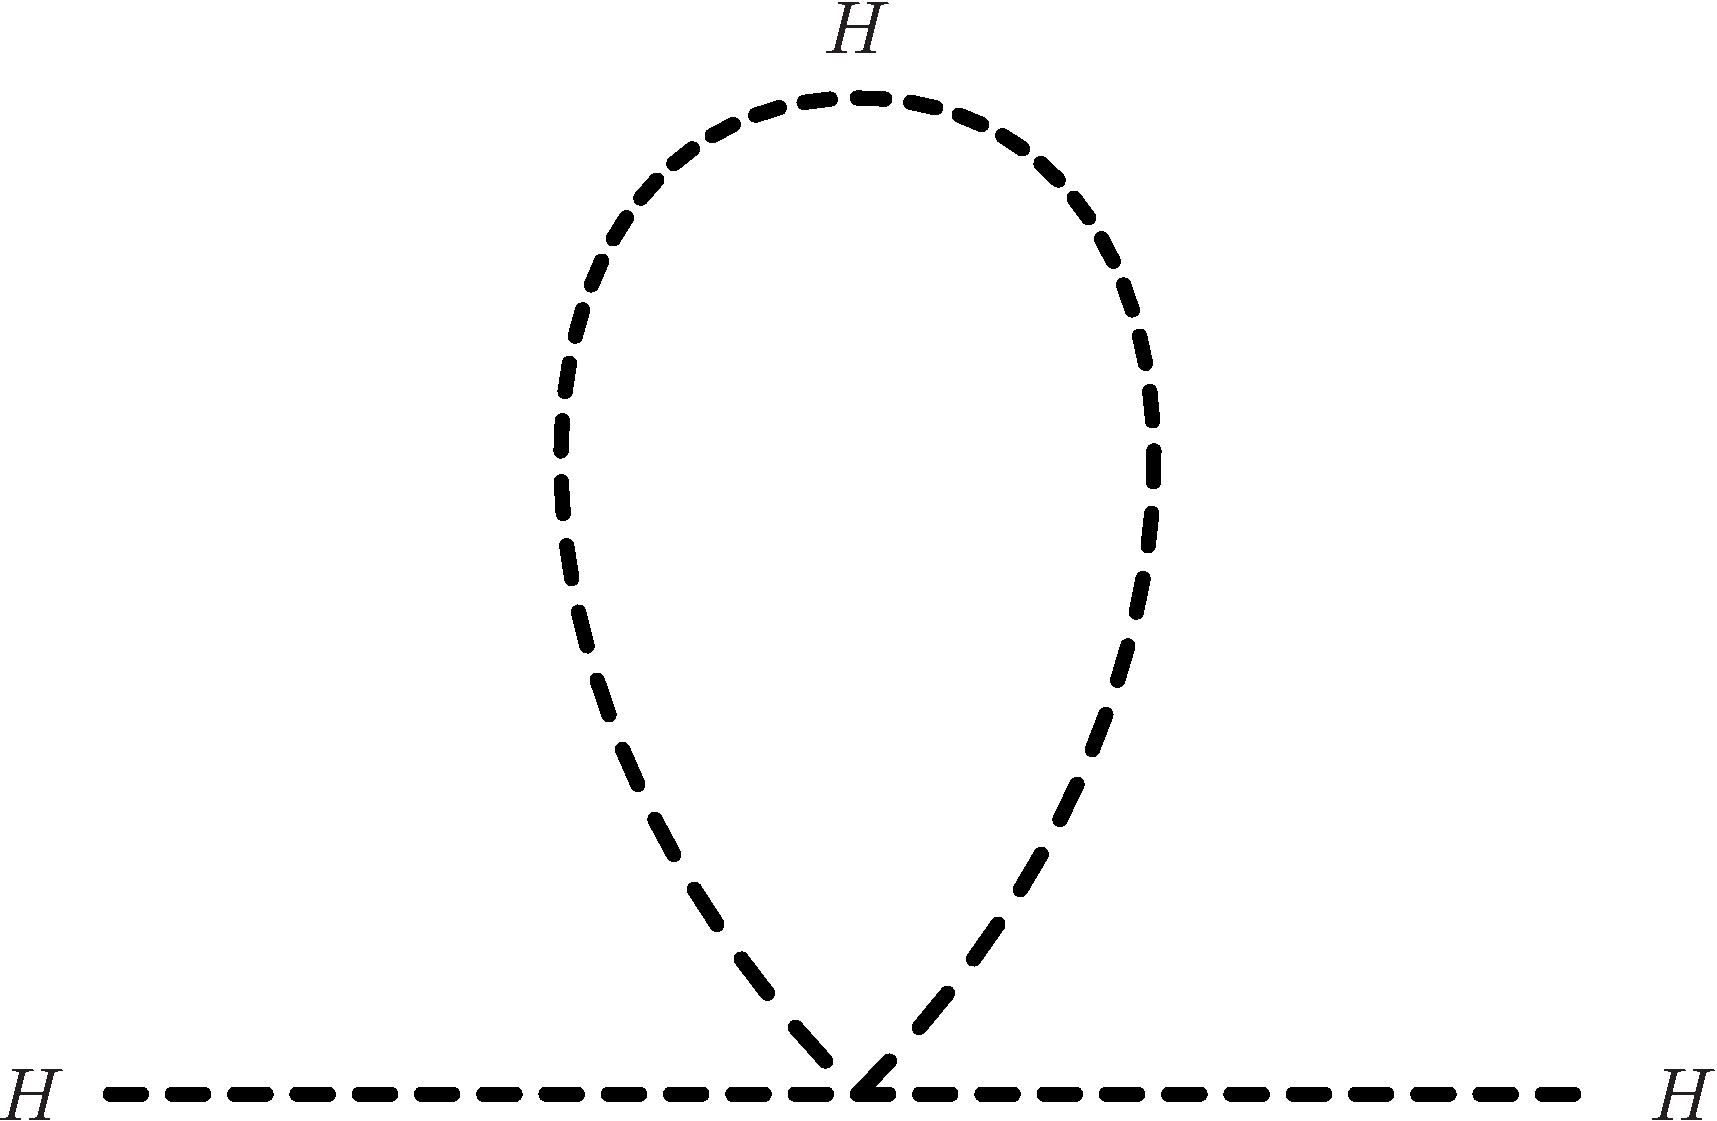
\includegraphics[width=0.3\textwidth]{\chtwo/HiggsLoop2.pdf}} 
 \caption{Radiative corrections to the Higgs squared mass parameter $m^2_\PH$ due to: (a) Yukawa coupling with the top quark; (b) gauge boson loop; (c) Higgs quartic self-interaction.}
 \label{fig:HiggsLoop}
\end{figure}

Many extensions of the SM suggest new physics at the TeV scale to address the hierarchy problem, providing more ``natural'' options.
Models of \textit{supersymmetry}~\cite{PhysRevD.24.1681,Casas:1994qy} introduce a new heavy scalar called \textit{stop} as \textit{superpartner} of the SM top quark,
which cancels out the top quark loop corrections to the Higgs mass. Non-supersymmetric models have also been proposed, which predict heavier partners to the top quark.
%In \textit{Little Higgs} models (Section~\ref{subsec:composite}), several heavy top quark partners (also called vector-like quarks) are introduced which cancel the quadratic divergence.
Another possibility to address the hierarchy problem is to assume the Higgs boson to be a composite particle as in the \textit{composite Higgs} models (Section~\ref{subsec:composite}),
rather than an elementary particle as predicted in the SM. %In these composite Higgs models, a Higgs boson may have decays as predicted by the SM. 

\subsection*{Dark matter and dark energy}

Several cosmological observations showed that the standard model only describes 5\% of the total content of the Universe.
First, the measured orbital velocities of stars around their galaxy center is incompatible with the observed matter density in the space.
In particular, assuming the gravitational mass is due to only visible matter, stars far from the center of galaxies have much higher velocities than expected. % (Fig.~\ref{fig:DarkMatter}).
The easiest way to account for this discrepancy is to postulate the existence of another kind of matter, called \textit{dark matter}, that does not interact through electromagnetic or strong interactions.
%\begin{figure}[!htb]
 %\centering
 %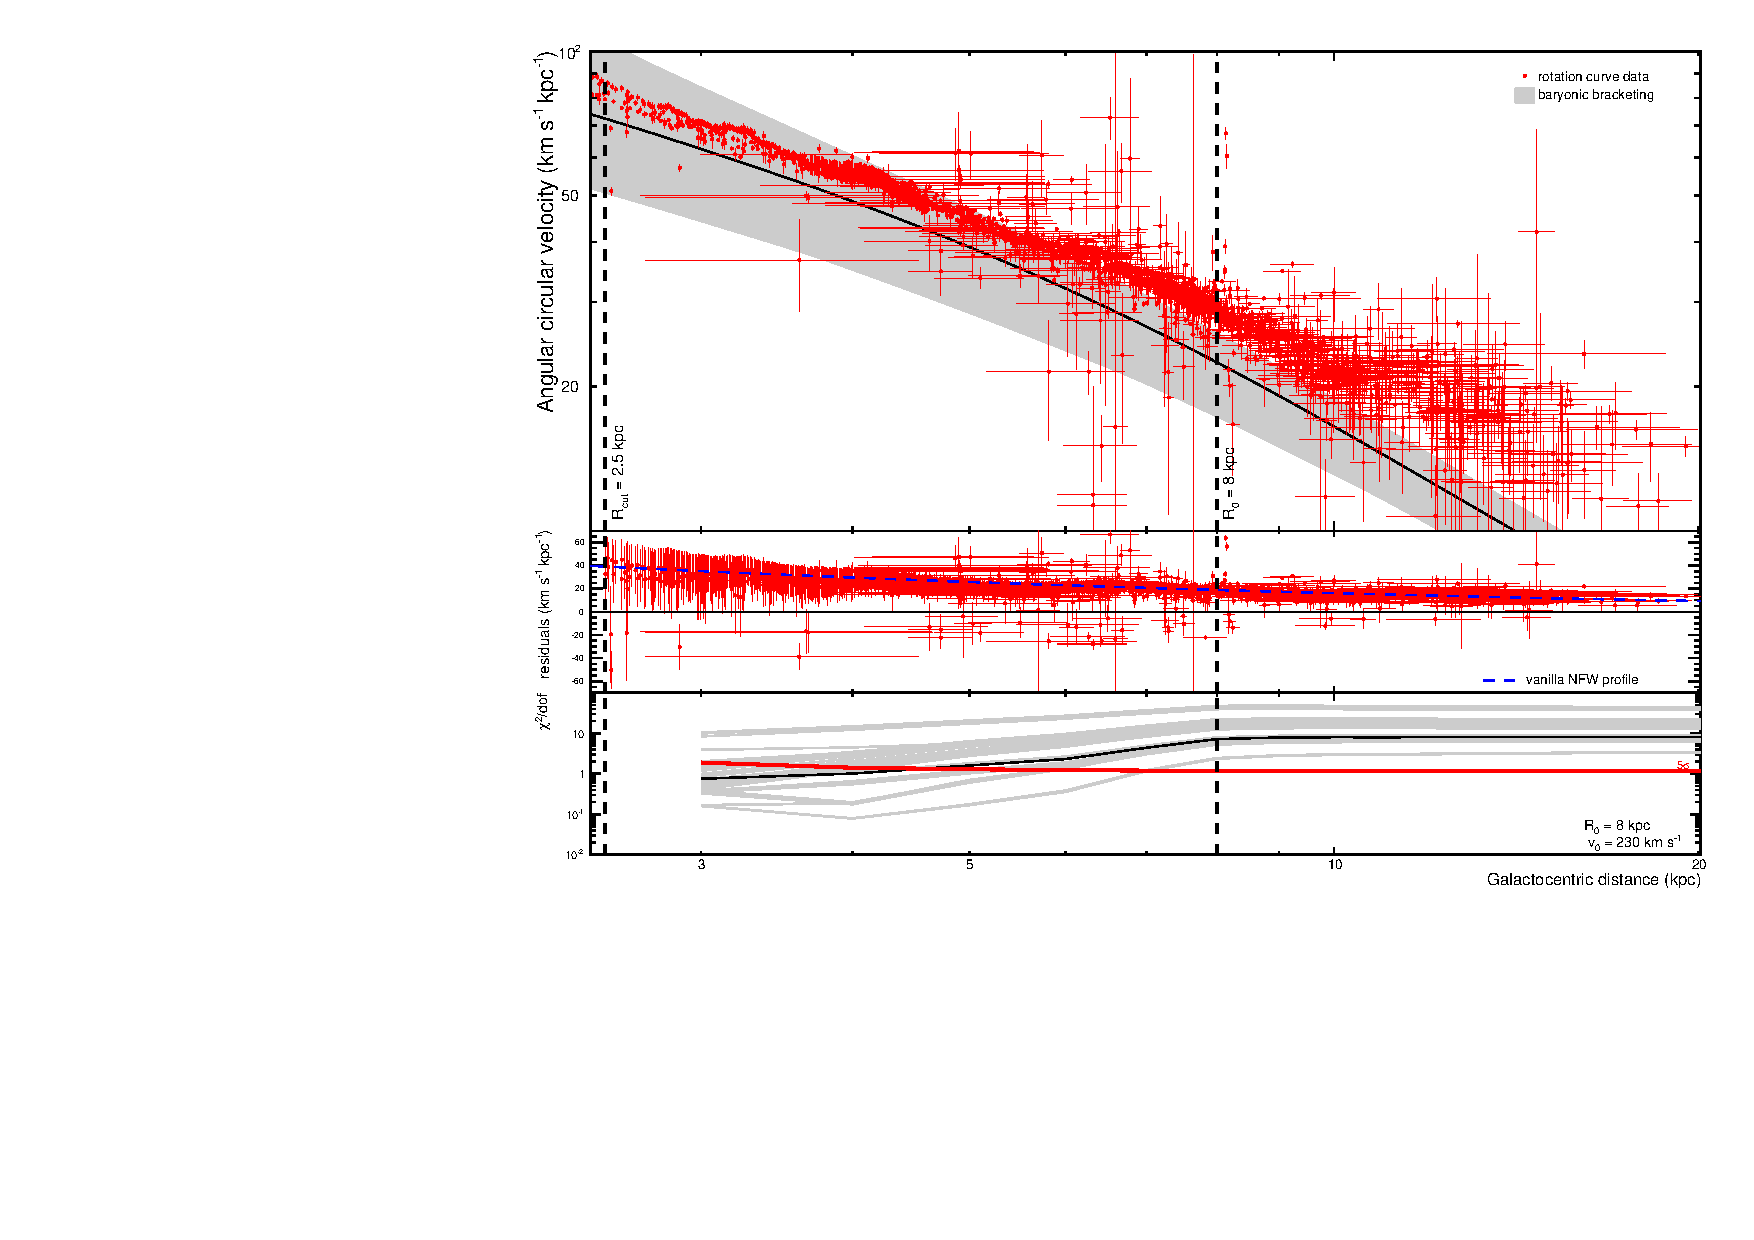
\includegraphics[width=0.6\textwidth]{\chtwo/wc_fit.pdf}
 %\caption{Measured rotation curve of the Milky Way representing the orbital velocities of visible stars or gas in that galaxy as a function of their radial distance from that galaxy's center. The contribution from visible matter is represented by the black line with its 1$\sigma$ uncertainty (grey band). The data strongly disfavor baryons as the sole contribution to the galactic mass budget~\cite{Iocco:2015xga}.}
 %\label{fig:DarkMatter}
%\end{figure}
A second major result in cosmology is the discovery that the Universe is in accelerated expansion: it was measured that in average galaxies recede from each other and that this escape rate increases with the distance.
Such a feature cannot be achieved with usual particles or with dark matter, whereas a new type of energy with a negative pressure, called \textit{dark energy}, has to be added to the Universe content.
To account for the experimental observations, dark matter and dark energy have been estimated to compose respectively 26\% and 69\% of the total Universe content~\cite{Ade:2015xua}, but their fundamental nature remains nowadays a mystery.
The most widely accepted hypothesis on the form for dark matter is that it is composed of weakly interacting massive particles (WIMPs) that interact only through gravity and the weak force.
The searches from the point of view of experimental and theoretical dark matter hunting is one of the major efforts in particle physics.
There are two fronts: direct searches in cosmic rays by underground experiments, and searches at hadron colliders, where dark matter would be produced in pairs of neutral particles that may be predicted by different models.
%In the case of supersymmetry, dark matter is incarnated by neutralinos ($\tilde{\chi}^0$), often called Weakly Interacting Massive Particles or WIMP's, in processes such as 
%\begin{equation*}
%p p \to X \to \tilde{\chi}^0 \tilde{\chi}^0
%\end{equation*}
No dark matter particle has been conclusively identified by any of these experiments.

\subsection*{Gravity}

The standard model does not include the fourth fundamental interaction, gravity.
In fact, gravity is by many aspects very different from the three other forces, and establishing a common framework to describe both raises several challenges.
In the decades after the discovery of general relativity, it was realized that general relativity is incompatible with quantum mechanics.
It is possible to describe gravity in the framework of quantum field theory like the other fundamental forces, such that the attractive force of gravity arises due to exchange of virtual spin-2 \textit{gravitons}, in the same way as the electromagnetic force arises from exchange of virtual photons. The theory arising from this approach is known as \textit{quantum gravity}.
%Moreover, whereas the strong, weak and electromagnetic forces have similar strengths at the electroweak scale, gravity is $10^{24}$ times weaker and becomes only appreciable for energies around the Planck scale.
This theory is known not to be renormalizable, as the loop corrections including a graviton induce divergencies that cannot be reabsorbed through the renormalisation procedure, as opposed to the electroweak and chromodynamics quantum theories. Thus, quantum gravity cannot be used to make meaningful physical predictions.
%Thus, a more complete theory of quantum gravity is required.
Moreover, quantum gravitational effects are only expected to become apparent near the Planck scale, a scale far smaller in distance (equivalently, far larger in energy) than what is currently accessible at high energy particle accelerators.
Several theoretical approaches to the problem of quantum gravity have been proposed, being one of the most popular the \textit{string theory}~\cite{StringTheory}.
%and \textit{loop quantum gravity}~\cite{Rovelli:2011eq}.

It has to be noted than most of these approaches only attempt to describe the quantum behavior of the gravitational field and should not be confused with the objective of unifying all fundamental interactions into a single mathematical framework. However, the present understanding of gravity would aid further work towards unification.
%A theory of quantum gravity that is also a grand unification of all known interactions is sometimes referred to as the \textit{theory of everything}.

%matter-antimatter asymmetry
%number of parameters
%number of flavors
%neutrino oscillations